%TOASK
%---------------------------------------------------------------------
%   documentclass
%---------------------------------------------------------------------
\documentclass[]{beamer}
% Class options include: notes, notesonly, handout, trans,
%                        hidesubsections, shadesubsections,
%                        inrow, blue, elcon-clr, grey, brown

%---------------------------------------------------------------------
%   packages
%---------------------------------------------------------------------
% Theme for beamer presentation.
\usepackage{beamerthemesplit}
% Other themes include: beamerthemebars, beamerthemelined,
%                       beamerthemetree, beamerthemetreebars
\usepackage[english]{babel}
\usepackage[enc=cp1250]{hrlatex}
\usepackage[T1]{fontenc} %pekne makcene
\usepackage{lmodern} %spolu s T1 smooth font!
\usepackage{cite} %bibtex
\usepackage[numbers]{natbib}
\usepackage{color} %for \textcolor{declared-color}{text}
\usepackage{floatflt} %to have tables and text beside
\usepackage{colortbl} %for \rowcolor command
\usepackage{scalefnt} %for scale font
\usepackage{pifont} %for ticks (check symbols)
\usepackage{pgfplots}
\usepackage{xcolor} %for \colorlet
\usepackage{lipsum}

\usepackage{tikz}
\usetikzlibrary{decorations.pathreplacing}

\colorlet{city-clr}{green!70!black}
\colorlet{elcon-clr}{red}
\colorlet{event-clr}{blue}
\colorlet{waiting-clr}{olive}
\colorlet{cmt-clr}{gray}
\colorlet{oracle-clr}{orange!30}

%---------------------------------------------------------------------
%   settings
%---------------------------------------------------------------------
\graphicspath{{./pics/}} %picture dir

\definecolor{tablehead}{RGB}{238,233,233} %nice smooth grey

\def\Tiny{ \font\Tinyfont = cmr10 at 3pt \relax  \Tinyfont}

\pgfrealjobname{presentation} % <-- NOTE: this needs to be the real document's basename
                        %     (else you'll only get an empty output file)

\newif\iffull
\fullfalse

\newif\iffinal % introduce a switch for draft vs. final document
\finaltrue % use this to compile the final document
\iffinal
  \newcommand{\inputTikZ}[1]{%
    \input{#1.tikz}%
  }
\else
  \newcommand{\inputTikZ}[1]{%
    \beginpgfgraphicnamed{#1-external}%
    \input{#1.tikz}%
    \endpgfgraphicnamed%
  }
\fi

%---------------------------------------------------------------------
%   environments
%---------------------------------------------------------------------
%\newcommand{\newblock}{}

\newcommand{\tick}{\ding{52}}
\newcommand{\cross}{\ding{55}}

%---------------------------------------------------------------------
%   theme
%---------------------------------------------------------------------
\usetheme{Darmstadt}
\usecolortheme{seahorse}

%---------------------------------------------------------------------
%   data
%---------------------------------------------------------------------
\title{\textbf{Oracles for timetable graphs}}
\subtitle{Or�kula pre grafy reprezentuj�ce cestovn� poriadky}
\author{\textbf{Franti�ek Hajnovi�}}
\institute{FMFI UK}
\date{\today}

%---------------------------------------------------------------------
%   document
%---------------------------------------------------------------------
\begin{document}

	%---------------------------------------------------------------------
	%   Title page
	%---------------------------------------------------------------------
	{
    \setbeamertemplate{background canvas}{
        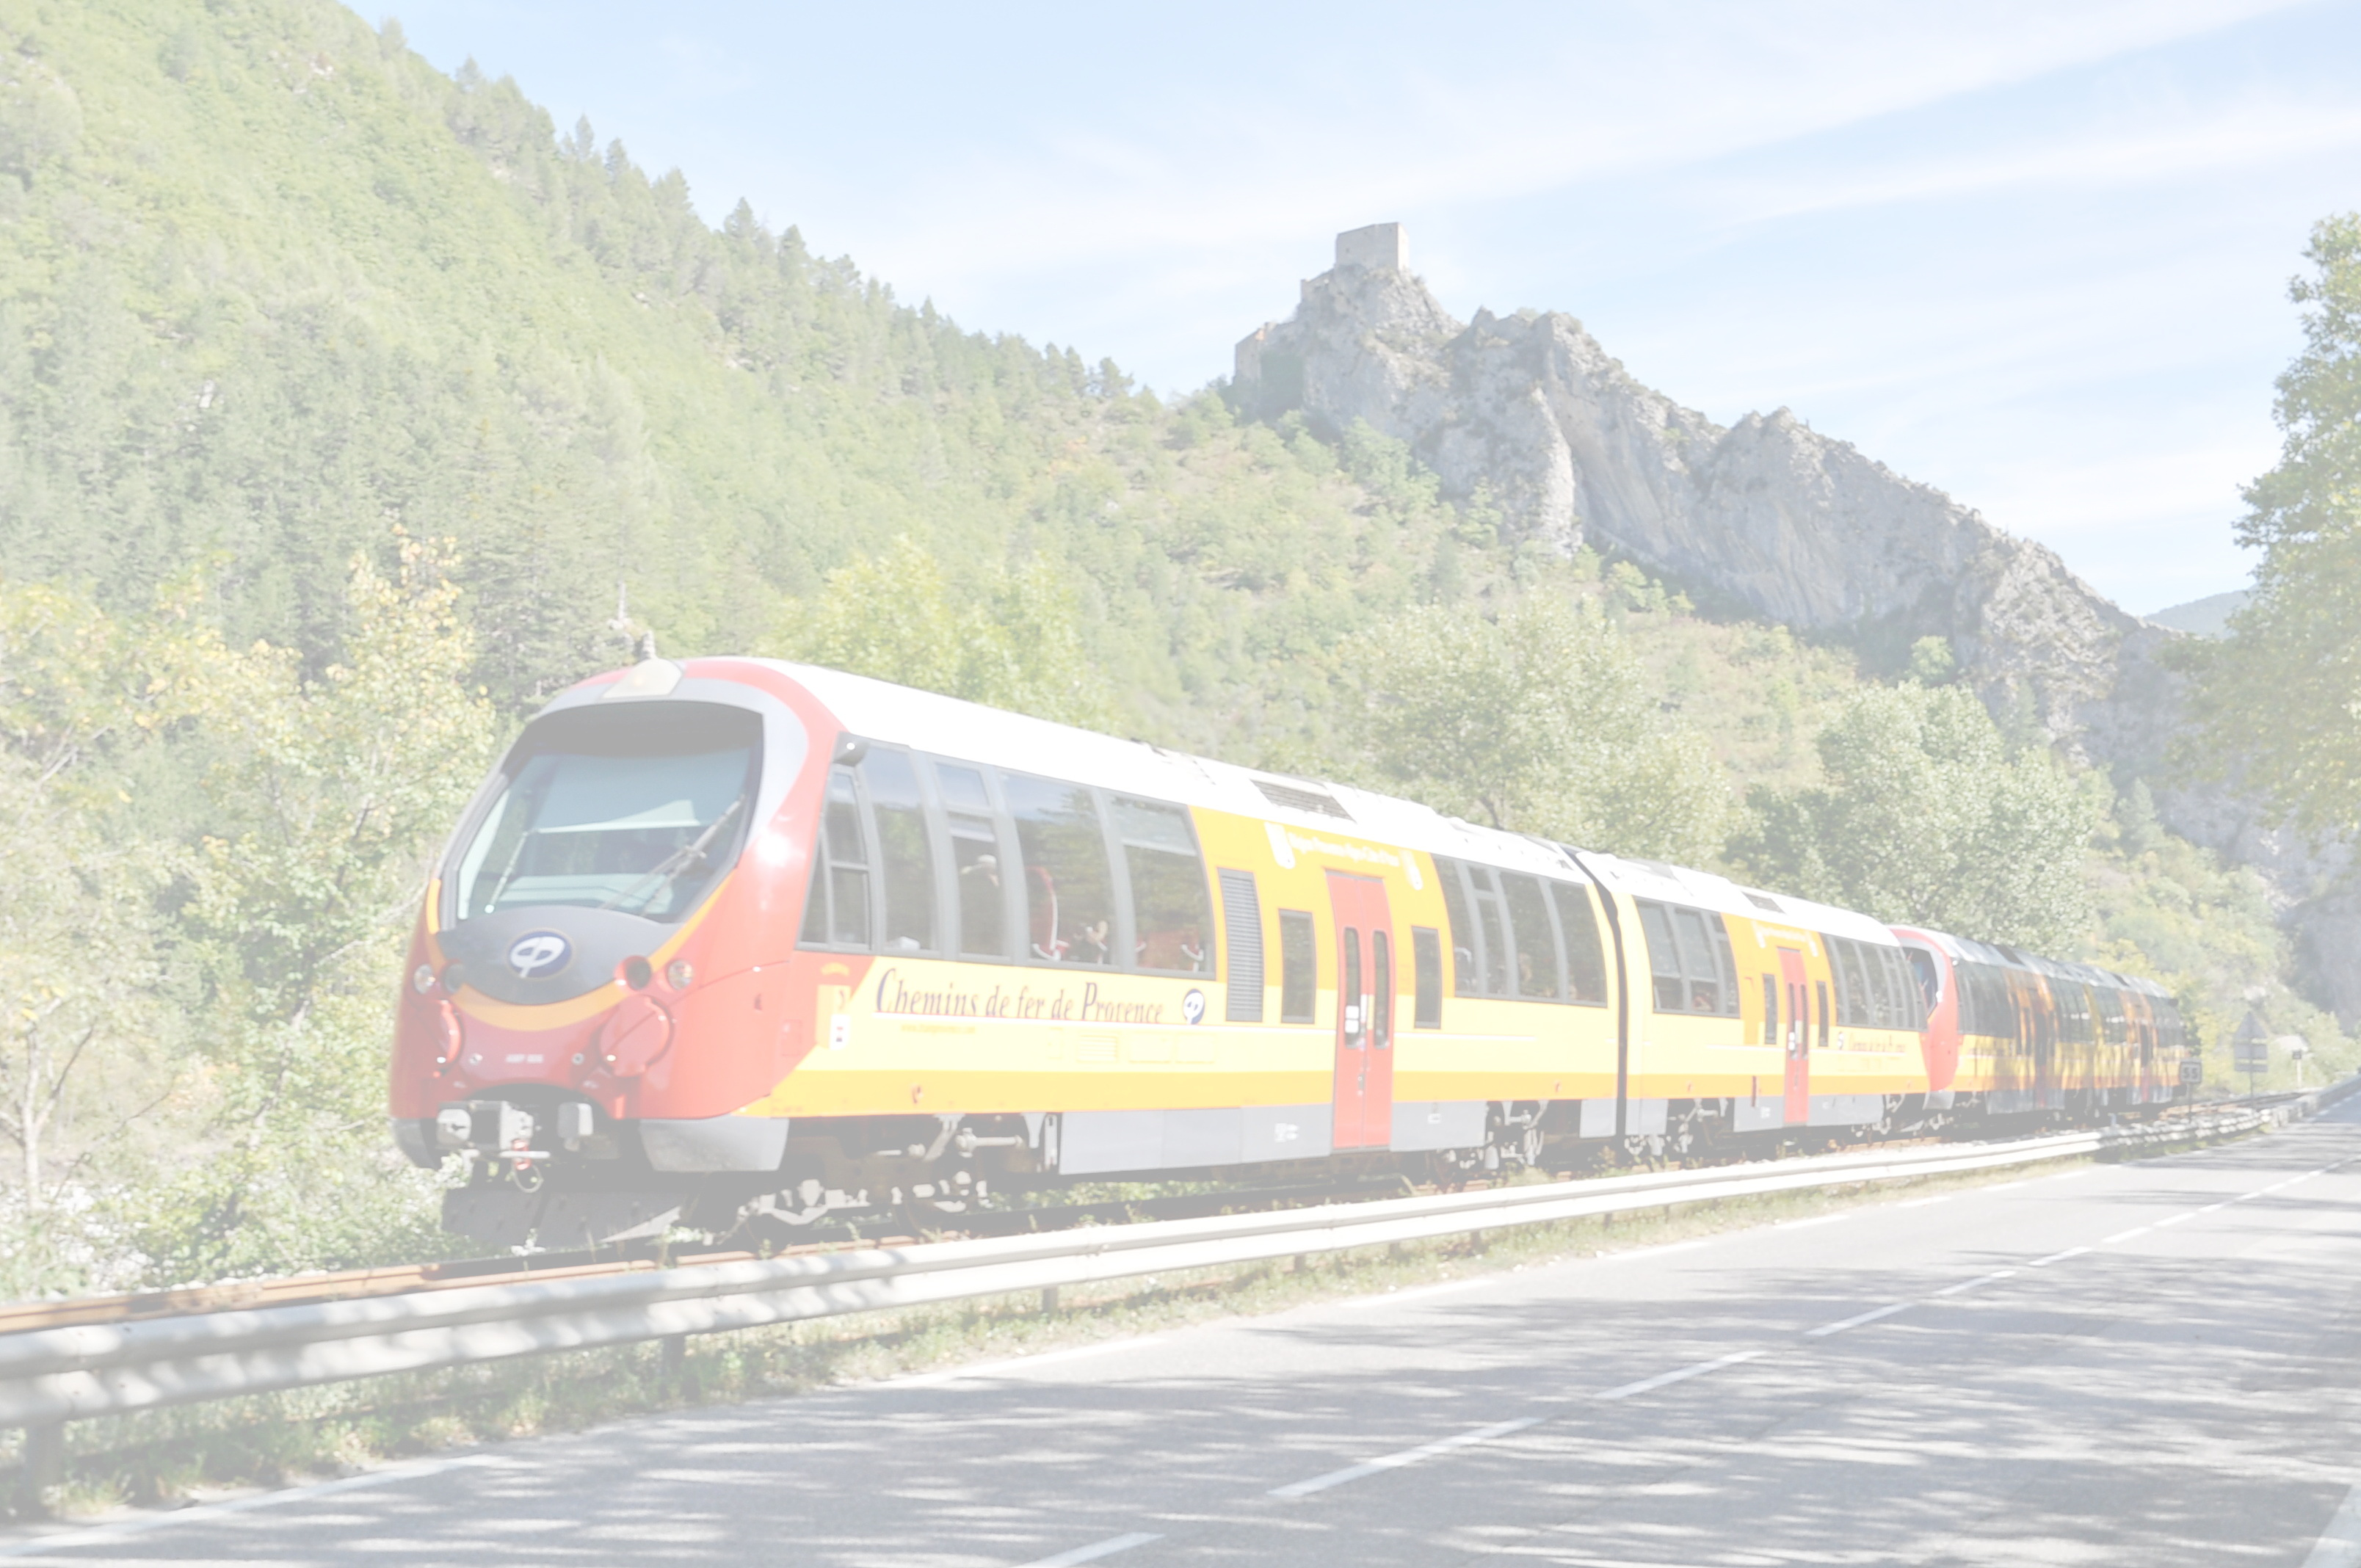
\includegraphics[height=\paperheight]{train.jpg}
    }
    \begin{frame}
        \titlepage
        \begin{center}
            Supervisor: \textit{doc. RNDr.} Rastislav Kr�lovi� \textit{PhD.}
        \end{center}
    \end{frame}
    }

	%---------------------------------------------------------------------
	%   Content
	%---------------------------------------------------------------------
    \begin{frame}
        \frametitle{Content}
        \tableofcontents
    \end{frame}

	%---------------------------------------------------------------------
	%   Introduction
	%---------------------------------------------------------------------
    \setbeamercolor{frametitle}{fg=elcon-clr!80!black}
    \section{Introduction}
    \begin{frame}
        \frametitle{Introduction}
        \begin{center}
            \textcolor{elcon-clr!80!black}{\textbf{Introduction}}
        \end{center}
    \end{frame}
    \setbeamercolor{frametitle}{fg=black!70}

		%---------------------------------------------------------------------
		%   What is it about?
		%---------------------------------------------------------------------
	    \begin{frame}
	        \frametitle{What is it about?}
	        \begin{itemize}
	            \item Given a timetable, we query - $(a, t, b)$ - for
	            \begin{itemize}
	            	\item \textbf{Earliest arrival} (EA) - $t_{(a, t, b)}^{*}$
	            	\item \textbf{Optimal connection} (OC) - $c_{(a, t, b)}^{*}$
	            \end{itemize}
	        \end{itemize}
	        \vspace{-0.5cm}
	        \begin{figure}[h!]
				\scriptsize
                \begin{center}
					\inputTikZ{./tikzpics/connection}
                \end{center}
            \end{figure}
            \vspace{-1cm}	
            \begin{itemize}
            	\item<2> \textbf{Motivation}
            	\begin{itemize}
            		\item<2> Large-scale timetable search engines (\emph{cp.sk, imhd.sk}...)
            	\end{itemize}
				\item<2> \textbf{Approach}
				\begin{itemize}
					\item<2> (Distance) oracle-based approach~\cite{apxdo05} - pre-computation
				\end{itemize}
			\end{itemize}
			\vspace{-0.5cm}
			\uncover<2>{\begin{figure}[h!]
                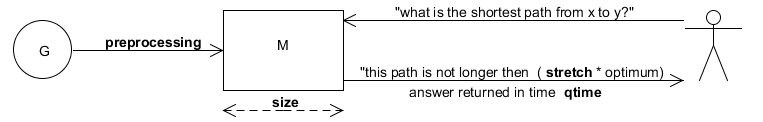
\includegraphics[height=0.5in]{dodiagram.png}
            \end{figure}}
	    \end{frame}
	    
	    %---------------------------------------------------------------------
        %   TT and UG graph
        %---------------------------------------------------------------------
        \begin{frame}
            \frametitle{Timetable and underlying graph}        
	        \begin{columns}[c]
            \column{2.7in}
				\begin{table}{
	                \scriptsize
	                \begin{tabular}{c|c|c|c}
	                %legend
	                    \hline
	                    \rowcolor{tablehead}
	                    \multicolumn{2}{>{\columncolor{tablehead}}c|}{\textbf{Place}} & \multicolumn{2}{>{\columncolor{tablehead}}c}{\textbf{Time}} \\
						\hline
	                    \rowcolor{tablehead}
	                    \textbf{From} & \textbf{To} & \textbf{Departure} & \textbf{Arrival} \\
	                %data
						\hline
	                    \textcolor{city-clr}{A} & \textcolor{city-clr}{B} & 10:00 & 10:45 \\
						\textcolor{city-clr}{B} & \textcolor{city-clr}{C} & 11:00 & 11:30 \\
						\textcolor{city-clr}{B} & \textcolor{city-clr}{C} & 11:30 & 12:10 \\
						\textcolor{city-clr}{B} & \textcolor{city-clr}{A} & 11:20 & 12:30 \\
						\textcolor{city-clr}{C} & \textcolor{city-clr}{A} & 11:45 & 12:15 \\
					\end{tabular}}
					\caption{\textbf{Timetable} - a set of \textcolor{elcon-clr}{\textbf{elementary connections}} (between pairs of \textbf{\textcolor{city-clr}{cities}})}
	            	\normalsize
				\end{table}
            \column{2.3in}
            	\begin{figure}[h!]
					\scriptsize
	                \begin{center}
						\inputTikZ{./tikzpics/ug}
	                \end{center}
                    \caption{\textbf{Underlying graph}}
                \end{figure}
			\end{columns}
			\begin{itemize}
				\item<2> \textbf{Goals}
				\begin{itemize}
	                \item<2> Devise methods to tackle EA/OC problem
		            \item<2> Analyse properties of timetables
	            \end{itemize}			
			\end{itemize}
		\end{frame}
		
	%---------------------------------------------------------------------
	%   Contribution 
	%---------------------------------------------------------------------
    \setbeamercolor{frametitle}{fg=elcon-clr!80!black}
    \section{Contribution}
    \begin{frame}
        \frametitle{Contribution}
        \begin{center}
            \textcolor{elcon-clr!80!black}{\textbf{Contribution}}
        \end{center}
    \end{frame}
    \setbeamercolor{frametitle}{fg=black!70}
    
	    %---------------------------------------------------------------------
        %   Data
        %---------------------------------------------------------------------
        \subsection{Data}
        \begin{frame}
            \frametitle{Data}
			\begin{table}{
                \tiny
                \begin{tabular}{c|c|c|c|c|c|c}
                %legend
                    \hline
                    \rowcolor{tablehead}
                    \textbf{Name} & \textbf{Description} & \textbf{El. conns.} & \textbf{Cities} & \textbf{UG arcs} & \textbf{Time range} & \textbf{Height ($h$)} \\
                %data
					\hline
					air01 & domestic flights (US) & 601489 & 287 & 4668 & 1 month & 24374 \\
					cpru & regional bus (SVK) & 37148 & 871 & 2415 & 1 day & 239 \\
					cpza & regional bus (SVK) & 60769 & 1108 & 2778 & 1 day & 370 \\
					montr & public transport (Montreal) & 7153 & 217 & 349  & 1 day & 363 \\
					sncf & country-wide rails (FRA) & 90676 & 2646 & 7994 & 1 day & 488 \\
					zsr & country-wide rails (SVK) & 932052 & 233 & 588 & 1 year & 60308 \\
				\end{tabular}}
				\caption{Timetables datasets}
            	\normalsize
			\end{table}
        \end{frame}

	    %---------------------------------------------------------------------
        %   Idea
        %---------------------------------------------------------------------
        \subsection{Underlying shortest paths}
        \begin{frame}
            \frametitle{Idea}
			\begin{itemize}
                \item \textit{``Usually we go through the same sequence of cities''}
            \end{itemize}
            \vspace{0.5cm}
            \begin{columns}[c]
            \column{2.7in}
            	\vspace{-1cm}
	            \begin{figure}[h]
					\scriptsize
	                \begin{center}
	                    \inputTikZ{./tikzpics/pathfunc}
	                \end{center}
	            \end{figure}
	            \vspace{-0.7cm}
	            \begin{itemize}
	            	\item $p$ is USP $\iff$ $\exists t: path(c_{(a, t, b)}^{*}) = p$
	            	\item we have USP $\rightarrow$ reconstruct $c_{(a, t, b)}^{*}$
	            	\item<2-> \textbf{Overtaking}~\cite{timetablemodelsalgs07} causes problems, but can be easily removed
	            \end{itemize}
	        \column{2.3in}
		        \vspace{-0.5cm}
	        	\begin{figure}[h!]
	                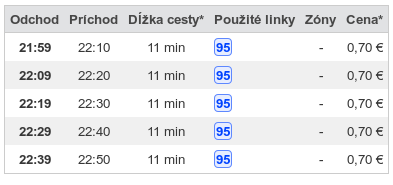
\includegraphics[height=0.9in]{redundancy.png}
	            \end{figure}
	            \uncover<2->{
	            	\vspace{-0.5cm}
	            	\begin{table}{
	                \tiny
	                \begin{tabular}{c|c}
	                %legend
	                    \hline
	                    \rowcolor{tablehead}
	                    \textbf{Name} & \textbf{Overtaken edges (\%)} \\
	                %data
						\hline
						air01 & 1\% \\
						cpru & 2\% \\
						cpza & 2\% \\
						montr & 1\% \\
						sncf & 2\% \\
						zsr & 0\% \\
					\end{tabular}}
	            	\normalsize
				\end{table}}
			\end{columns}
        \end{frame}
        
        %---------------------------------------------------------------------
        %   USP-OR
        %---------------------------------------------------------------------
        \begin{frame}
            \frametitle{USP-OR}
            \begin{columns}[c]
            \column{2.9in}
				\begin{itemize}
					\small
					\item<1-> Pre-compute \textit{all conn.} - space $\mathcal{O}(h \; n^{3})$
					\begin{itemize}
	                	\item daily height usually $200$ < $h$ < $800$
	                \end{itemize}
	                \item<2-> Pre-compute \textit{all USPs} - space $\mathcal{O}(\tau \; n^{3})$
	                \begin{itemize}
	                	\item $\tau_{A, B}$ - \# of USPs between $A$ and $B$
	                \end{itemize}
	            \end{itemize}
	            \uncover<3->{\begin{table}{
	                \scriptsize
	                \begin{tabular}{c|c|c|c}
	                %legend
	                    \hline
	                    \rowcolor{oracle-clr}
	                    \textbf{Prep-time} & \textbf{Size} & \textbf{Q-time} & \textbf{Stretch} \\
	                %data
						\hline
						$\mathcal{O}(hn^{3})$ & $\mathcal{O}(\tau \; n^{3})$ & $\mathcal{O}(\tau \; n)$ & $1$ \\
					\end{tabular}}
					\caption{USP-OR parameters}
	            	\normalsize
				\end{table}}
				\vspace{-0.5cm}
				\begin{itemize}
					\item<3> $\tau$ almost constant, USP size $\approx \sqrt{n}$
					\item<3> Space $\mathcal{O}(n^{2.5})$ too big anyway
				\end{itemize}
	        \column{2.1in}
	        	\uncover<2->{\begin{table}{
	                \scriptsize
	                \begin{tabular}{c|c|c}
	                %legend
	                    \hline
	                    \rowcolor{tablehead}
	                    \textbf{Name} & \textbf{avg $\tau_{A, B}$} & \textbf{max $\tau_{A, B}$} \\
	                %data
						\hline
						air01 & 5.8 & 30 \\
						cpru & 7.0 & 64 \\
						cpza & 5.1 & 42 \\
						montr & 4.3 & 30 \\
						sncf & 4.3 & 24 \\
						zsr & 2.5 & 19 \\
					\end{tabular}}
					\caption{\footnotesize Daily, 200 station timetables}
	            	\normalsize
				\end{table}}
				\vspace{-0.7cm}
				\uncover<2->{\begin{table}{
	                \scriptsize
	                \begin{tabular}{c|c}
	                %legend
	                    \hline
	                    \rowcolor{tablehead}
	                    \textbf{Name} & \textbf{avg USP size} \\
	                %data
						\hline
						air01 & 3.0 \\
						cpru & 13.8 \\
						cpza & 11.1 \\
						montr & 20.3 \\
						sncf & 10.5 \\
						zsr & 13.7 \\
					\end{tabular}}
					\caption{\footnotesize Daily, 200 station timetables}
	            	\normalsize
				\end{table}}
	        \end{columns}
        \end{frame}
        
        %---------------------------------------------------------------------
        %   USP-OR - grafy
        %---------------------------------------------------------------------
        \begin{frame}
            \frametitle{USP-OR - $\tau$ evolution}
            \begin{columns}[c]
            \column{2.4in}
				\begin{figure}[h]
					\scriptsize
	                \begin{center}
	                    \inputTikZ{./tikzpics/plot_usp_air01_timerange}
	                \end{center}
	                \caption{\footnotesize Changing of $\tau$ with increased time range in \textit{air01} dataset. 1 day = about 800 in height}
	            \end{figure}
	        \column{2.4in}
	        	\begin{figure}[h]
					\scriptsize
	                \begin{center}
	                    \inputTikZ{./tikzpics/plot_usp_sncf_size}
	                \end{center}
	                \caption{\footnotesize Changing of $\tau$ with increased \# of stations in \textit{sncf} dataset}
	            \end{figure}
	        \end{columns}
        \end{frame}
        
        %---------------------------------------------------------------------
        %   USP-OR-A
        %---------------------------------------------------------------------
        \begin{frame}
            \frametitle{USP-OR-A}
		    \footnotesize
			\begin{itemize}
				\item Pre-compute USPs only among \textit{some} cities in UG: set of \textbf{access nodes} $\mathcal{A}$
				\item We would like ($r1$ and $r2$ small constants w.r.t. $n$):
				\begin{itemize}
					\footnotesize
					\item Size $|\mathcal{A}| = \mathcal{O}(\sqrt{n})$
					\item Small node neighbourhoods: $\forall v \; |neigh_{\mathcal{A}}(v)| < r_1 \cdot \sqrt{n}$
					\item Few local access nodes: $\forall v \; |lan_{\mathcal{A}}(v)| \leq r_2$
				\end{itemize}
	        \end{itemize}
	        \vspace{-0.2cm}
	        \makebox[\linewidth]{\parbox{12cm}{\begin{figure}[h]
				\scriptsize
                \begin{center}
					\inputTikZ{./tikzpics/uspora}
                \end{center}
			\caption{\footnotesize \textbf{1.)} Local search of $neigh_{\mathcal{A}}(A)$, \textbf{2.)} All-pairs USPs, \textbf{3.)} Local search \textit{against} $b$-$neigh_{\mathcal{A}}(B)$}
            \end{figure}}}
        \end{frame} 
        
        %---------------------------------------------------------------------
        %   Searching for ANs
        %---------------------------------------------------------------------
        \begin{frame}
            \frametitle{Searching for optimal AN set}
            \begin{columns}[c]
            \column{2.5in}
				\begin{itemize}
					\item NP-complete
					\begin{itemize}
						\item Reduction to min-set-cover
					\end{itemize}
				\end{itemize}
			\column{2.5in}
				\begin{figure}[h!]
	                
\includegraphics[height=0.6in]{ttblazer.png}
	                \caption{text}
	            \end{figure}
			\end{columns}
			\begin{itemize}
				\item<2> Heuristics: node $v$ with low $|neigh_{\mathcal{A}}(v) \cap b$-$neigh_{\mathcal{A}}(v)|$ but high $\min\{|neigh_{\mathcal{A}}(v)|, |b$-$neigh_{\mathcal{A}}(v)|\}$ is good ANs
			\end{itemize}
        \end{frame}
        
        %---------------------------------------------------------------------
        %   Existing methods
        %---------------------------------------------------------------------
        \begin{frame}
            \frametitle{Existing methods}
			\begin{itemize}
				\item \textbf{Time-dependent SHARC} \cite{sharc08}, \textbf{Time-dependent CH} \cite{timedepch09}
				\begin{itemize}
					\item Speed-ups of about 26 / 1500, respectively (EA only)
					\item Meant for time-dependent routing in road networks
				\end{itemize}
				\item \textbf{Time-expanded approach} \cite{engtimeexp09}
				\begin{itemize}
					\item Speed-ups of about 56
					\item Remodelling unimportant stations
				\end{itemize}
				\item \textbf{Theory vs. practice} difference
				\begin{itemize}
					\item Inclusion of transfers, cost...
				\end{itemize}
			\end{itemize}
        \end{frame}            
      
        %---------------------------------------------------------------------
        %   NN
        %---------------------------------------------------------------------
        \subsection{Neural networks}
        \begin{frame}
            \frametitle{Neural network approaches}
			\begin{itemize}
				\item Multi-layer perceptron, back propagation
				\item Input layer = \textcolor{event-clr}{events} + \textcolor{city-clr}{cities}. Output layer:
				\begin{enumerate}
					\item Arcs of UG $\rightarrow$ USP
					\item Arcs of UG $\rightarrow$ routing
					\item Earliest arrival value
				\end{enumerate}
			\end{itemize}
			\begin{figure}[h]
				\scriptsize
                \begin{center}
                    \inputTikZ{./tikzpics/neural}
                \end{center}
				\caption{Approach 1.)}
            \end{figure}
        \end{frame}  
        
        %---------------------------------------------------------------------
        %   Results
        %---------------------------------------------------------------------
        \begin{frame}
            \frametitle{Results}
			\begin{itemize}
				\item Tendency to remember USPs
				\item Long training times
			\end{itemize}            
			\begin{table}{
                \scriptsize
                \begin{tabular}{c|c|c|c}
                %legend
                    \hline
                    \rowcolor{tablehead}
                    \textbf{Name} & \textbf{Conn.} & \textbf{Found} & \textbf{Was optimum (\%)} \\
                %data
					\hline
					air01 & 931 & 573 & 18.7\% \\
					cpru & 481 & 281 & 48\% \\
					montr & 527 & 346 & 86.7\% \\
					zsr & 672 & 307 & 76.2\% \\
				\end{tabular}}
				\caption{Tests of a trained NN on timetables with 30 cities (approach 1.)}
            	\normalsize
			\end{table}
        \end{frame}
       
        %---------------------------------------------------------------------
        %   TTBlazer
        %---------------------------------------------------------------------
        \subsection{TTBlazer application}
        \begin{frame}
            \frametitle{Timetable analyzer - TTBlazer}
			\begin{itemize}
				\item Works with UG, TE, TD, TT
				\item Analysis ($\tau$, HD, degrees...), oracles (USP-OR, Dijkstra...), modifications (remove overtaking...), generation (subgraphs, TT $\rightarrow$ TD ...)
				\item Running \& evaluating tests
				\item Easily extendible
			\end{itemize}
			\begin{figure}[h!]
                
\includegraphics[height=0.6in]{ttblazer.png}
                \caption{It's \textit{blazing} fast!}
            \end{figure}
        \end{frame}	
    
    %---------------------------------------------------------------------
	%   Conclusion
	%---------------------------------------------------------------------
    \setbeamercolor{frametitle}{fg=elcon-clr!80!black}
    \section{Conclusion}
    \begin{frame}
        \frametitle{Conclusion}
        \begin{center}
            \textcolor{elcon-clr!80!black}{\textbf{Conclusion}}
        \end{center}
    \end{frame}
    \setbeamercolor{frametitle}{fg=black!70}
    
    	%---------------------------------------------------------------------
        %   Conclusion
        %---------------------------------------------------------------------
        \begin{frame}
            \frametitle{Conclusion}
			\begin{itemize}
				\item Trying out novel approaches to solving EAP in timetables
				\begin{itemize}
					\item \textit{USP-OR}: Exact and quick answers but high space and time preprocessing
					\item \textit{NN}: Problem too challenging for NN/try different types of network
				\end{itemize}
				\item Analysis of \textbf{various} real-world timetables
				\begin{itemize}
					\item Better insight on properties of timetables
				\end{itemize}
				\item Useful and easily extendible application
			\end{itemize}
        \end{frame}
        
%---------------------------------------------------------------------
%   Bibliography
%---------------------------------------------------------------------
    \begin{frame}[allowframebreaks]
        \frametitle{Bibliography}
        \tiny
        \bibliographystyle{is-alpha}
        \bibliography{../bibl}
        %compile latex, bibtex, latex, latex
    \end{frame}

%---------------------------------------------------------------------
%   Thanks for the attention
%---------------------------------------------------------------------
	{
    \setbeamertemplate{background canvas}{
        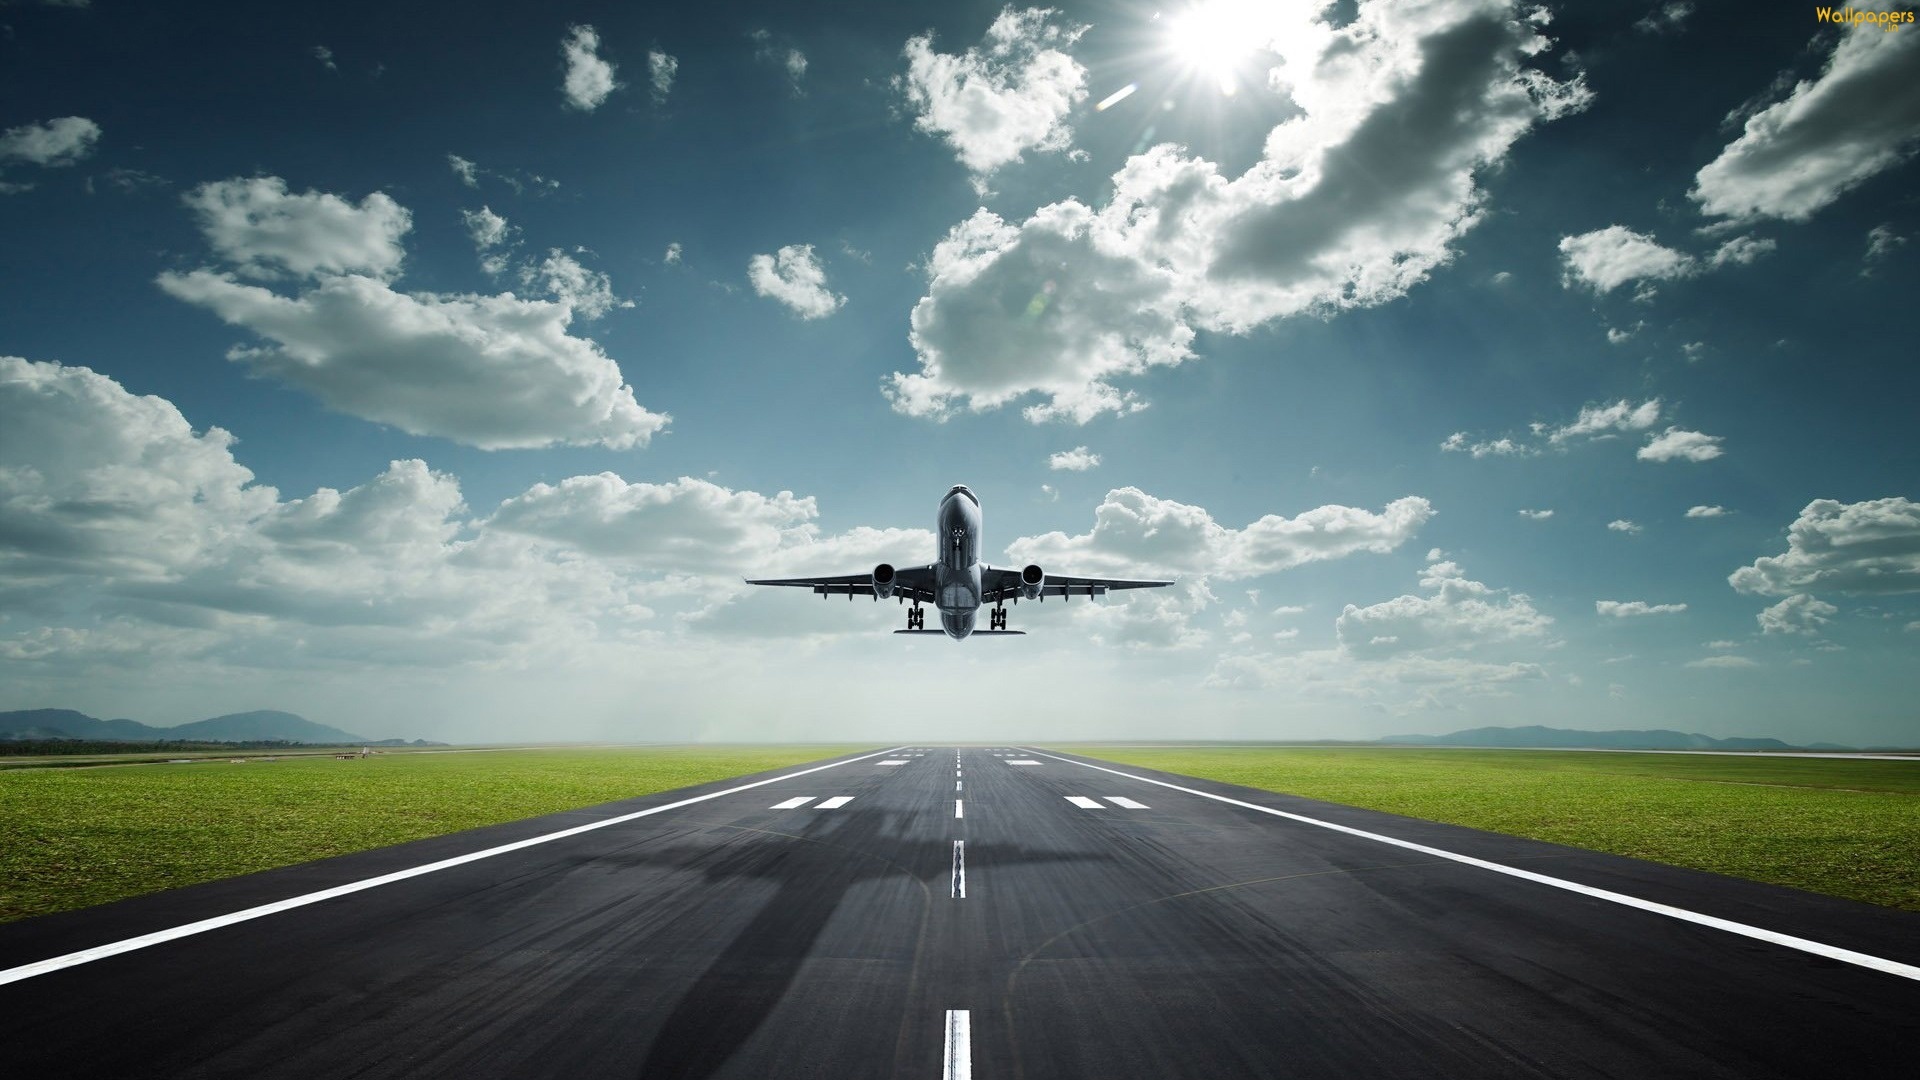
\includegraphics[height=\paperheight]{takeoff.jpg}
    }
    \begin{frame}
        \frametitle{Thank you for the attention}
        \begin{center}
        	\vskip 2cm
            \textbf{Thank you for the attention}
        \end{center}
    \end{frame}
    }

\end{document}
